\subsection{Utliggerdeteksjon}
Om et måleinstrument er upresist kan vi anta at målesignalene er utsatt for Gaussisk støy, og likevel få nyttig informasjon fra hver observasjon $y_i = f(x_i) + \varepsilon_i$. Det er imidlertid ikke alle feil som er fullt så hyggelige. En feil inntasting av data er vanskelig å modellere som noe annet enn feil som ideelt sett burde fjernes, og korrekte målinger av ekstreme tilfeller kan gjøre mer skade enn nytte når man vil ha en modell som stort sett fungerer. Disse to tilfellene ville antagelig hatt hhv. høy \textit{residual} og \textit{leverage}, vist i figur \ref{fig:utliggere}.

\begin{figure}[h]
	\centering
	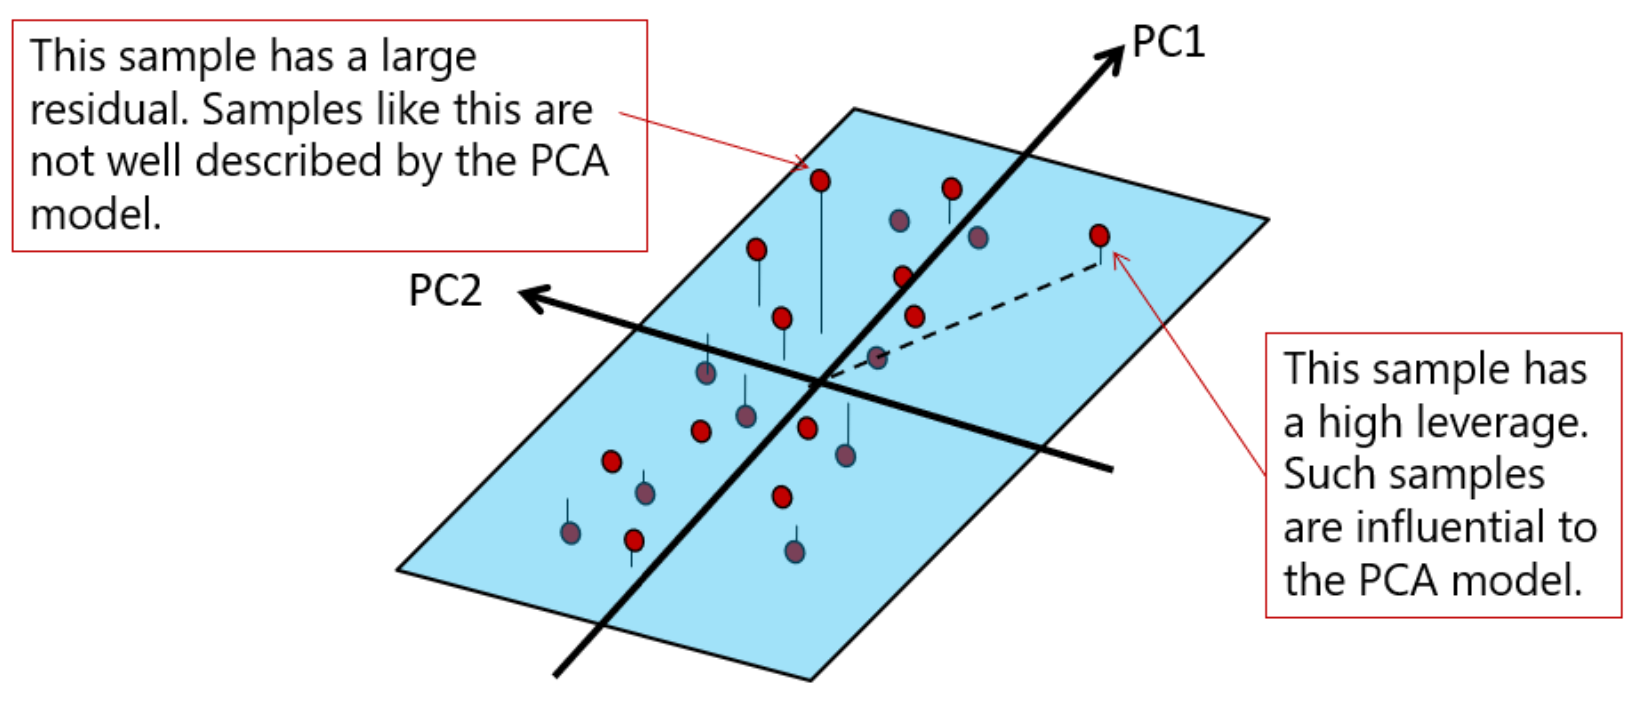
\includegraphics[width=0.8\textwidth]{figurer/utligger_illustrasjon.png}
	\caption{Ulike typer utliggere}
	\label{fig:utliggere}
\end{figure}

La $T$ være en matrise med scores slik at $X \approx T P^T$. Et mål på ``utliggerhet'' er bør da si noe om avstand til ``resten av dataen''. Noen slike verdier følger.

\subsubsection{Hotellings $T^2$}
\textbf{Hotellings} $T^2$ representerer avstanden til modellsenter i modellrommet (definert av $T$). For en observasjon $y_n$ er

\begin{equation}
	T_n^2 = \sum_{a=1}^A (t_{na} (T_a ^T T_a)^{-1} t_{na}^T) (n-1)
	\label{eq:hotelling_T2}
\end{equation}

$T^2$ er F-fordelt, og kan dermed brukes til å finne ut om $y_n$ kommer fra samme populasjon som resten av observasjonene (med et eller annet signifikansnivå). En typisk måte å visualisere dette på er som en ellipse i et score-plott. 

\subsubsection{Leverage}
For observasjonen $y_n$ er \textbf{leverage} gitt av

\begin{equation}
	h_n = \frac{1}{N} + t_{n, 1:A} (T_{1:A}^T T)^{-1} t_{n, 1:A}^T
\end{equation}
For leverage brukes vanligvis ikke signifikans for å bestemme kritisk grense (dvs. hva som defineres som en utligger), men heller en definisjon som er ganske så ad-hoc: $h_{\textrm{kritisk}} = \frac{3(A+1)}{N}$.

Summen av $h_n$ over alle $n$ observasjoner er 1, så leverage kan sees på som andelen varians en observasjon bidrar med. Denne verdien er lineært avhengig av Hotellings $T^2$ gjennom formelen

\begin{equation}
	T^2 = (N-1) (h - \frac{1}{N})
\end{equation}

\subsubsection{F- og Q-Residualer}
Som tidligere beskrevet er residualene for en modell $T P^T$ tilpasser $X$ gitt av

\begin{equation}
	E_A = X - \sum_{a = 1}^A t_a p_a^T
\end{equation}
der $A$ er antall PC-er brukt i modellen. For en enkelt observasjon $x_{nk}$ er residualen (gitt samme modell) gitt av

\begin{equation}
	e_{nk, A} = x_{nk} - \sum_{a = 1}^A t_{na} (p^T)_{ak}
\end{equation}

Disse gir ulike måter å representere residualene på. Om man er interessert i å undersøke enkeltobservasjoner (som gir mening siden utliggere jo er observasjoner) kan kritiske grenser for $e_{nk, A}$ estimeres vha. F- eller Q-fordelingen. 

\textbf{Q-residualen} er gitt av

\begin{equation}
	Q_{i, A} = e_{n, A}^T e_{n, A}
\end{equation}
og om man ønsker å finne kritisk Q-verdi for signifikans $\alpha$, kan man finne $c_\alpha$ i en tabell for standardnormalfordelingen, og bruke denne saftige formelen

\begin{equation}
Q_{a}=\theta_{1}\left(\frac{c_{a} \sqrt{2 \theta_{2} h_{0}^{2}}}{\theta_{1}}+\frac{\theta_{2} h_{0}\left(h_{0}-1\right)}{\theta_{1}^{2}}+1\right)^{\frac{1}{h_{0}}}
\end{equation}
der $\theta_1 = \textrm{trace}(E)$, $\theta_2 = \textrm{trace}(E^2)$, $\theta_3 = \textrm{trace}(E^3)$ og $h_0 = 1 - \frac{2 \theta_1 \theta_3}{3 \theta_2^2}$.

F-residualen kan finnes vha. Q-residualen, og regnes som mer konservativ. Den er gitt av

\begin{equation}
	F_{i, A} = \frac{Q_i}{K}
\end{equation}
Når man kjenner denne kan man gjennomføre en vanlig F-test.

Om man ikke vil bruke formler og finne disse verdiene manuelt, kan man bruke de innebygde metodene for dette som antageligvis allerede eksisterer i \texttt{verkøytet} man bruker for dataanalyse.

\subsubsection{Plott}
Det finnes mange nyttige plott man kan bruke når man vil oppdage utliggere, typisk i form av scatterplot med grensene diskutert i dette avsnittet plottet som linjer eller kurver. Kan hende kommer det noen figurer her etter hvert, eller kanskje et lite eksempel.
